% !TEX program = xelatex
% !BIB program = bibtex

\documentclass[UTF8]{article}

% layout
\usepackage[left=3cm,right=3cm]{geometry}
\usepackage{paralist} % for compactitem environment
\linespread{1.25}
% \makeatletter
% \def\@seccntformat#1{%
%   \expandafter\ifx\csname c@#1\endcsname\c@section
%   Section \thesection:
%   \else
%   \csname the#1\endcsname\quad
%   \fi}
% \makeatother
 
% page headings
\usepackage{fancyhdr}
\setlength{\headheight}{15.2pt}
\pagestyle{fancy}
\lhead{\leftmark}
\rhead{M201873026 Yilong Liu}
\cfoot{\thepage}
% \makeatletter
% \let\headauthor\@author
% \makeatother

% url/ref
\usepackage{hyperref}
\hypersetup{
  colorlinks,
  citecolor=black,
  filecolor=black,
  linkcolor=black,
  urlcolor=black,
  pdfauthor={Yilong Liu},
  pdftitle={Dataflow architecture: state-of-the-art and research challenges}
}

% vertical centering title page
\usepackage{titling}
\renewcommand\maketitlehooka{\null\mbox{}\vfill}
\renewcommand\maketitlehookd{\vfill\null}

% table of contents
\usepackage{tocloft}
\renewcommand\cftsecfont{\normalfont}
\renewcommand\cftsecpagefont{\normalfont}
\renewcommand{\cftsecleader}{\cftdotfill{\cftsecdotsep}}
\renewcommand\cftsecdotsep{\cftdot}
\renewcommand\cftsubsecdotsep{\cftdot}
\renewcommand{\contentsname}{\hfill\bfseries\Large Contents\hfill}   
\setlength{\cftbeforesecskip}{10pt}

% figures
\usepackage{graphicx}
\graphicspath{figures/}
% \newcommand\figureht{\dimexpr
%   \textheight-3\baselineskip-\parskip-.2em-
%   \abovecaptionskip-\belowcaptionskip\relax}

% tables
\usepackage{caption} 
\captionsetup[table]{skip=10pt}

% math, algorithms, code
\usepackage{amsmath,amssymb,url}
\usepackage{algorithm,algorithmicx,algpseudocode}
\usepackage{listings}

\lstset{
   extendedchars=true,
   basicstyle=\footnotesize\ttfamily,
   showstringspaces=false,
   showspaces=false,
   numbers=left,
   numberstyle=\footnotesize,
   numbersep=9pt,
   tabsize=2,
   breaklines=true,
   showtabs=false,
   captionpos=b
}

% bibliography
\usepackage[super,square,comma,sort]{natbib} % for \citet and \citep
\renewcommand{\refname}{References}
% \begin{filecontents}{report.bib}
% \end{filecontents} 

% appendix
\usepackage{appendix}

\title{Survey \\ \bigskip \textbf{Dataflow architecture: state-of-the-art and research challenges}}
\author{School of computer science and technology\\ M1801\\ M201873026\\ Yilong Liu}
\date{\today}

\begin{document}

\pagenumbering{gobble} % no page number
\maketitle
\newpage
% \null\thispagestyle{empty}
% \newpage

% \pagenumbering{roman}
% \section*{Abstract}\sectionmark{Abstract}
% \addcontentsline{toc}{section}{Abstract}
% \addcontentsline{toc}{section}{\protect\numberline{}Abstract}
% \newpage
% \pagenumbering{gobble} % no page number

\tableofcontents
\newpage
% \null\thispagestyle{empty}
% \newpage

\pagenumbering{arabic}

\section{Introduction}
Dataflow architecture is a computer architecture that
directly contrasts the traditional von Neumann architecture
or control flow architecture.
Dataflow architectures do not have a program counter,
or (at least conceptually) the executability
and execution of instructions is solely determined
based on the availability of input arguments to the instructions,
so that the order of instruction execution is unpredictable.
Dataflow architectures that are deterministic in nature
enable programmers to manage complex tasks
such as processor load balancing, synchronization and accesses to common resources.

The research, however, never overcame the problems related to:
\begin{compactitem}
  \item Efficiently broadcasting data tokens in a massively parallel system;
  \item Efficiently dispatching instruction tokens in a massively parallel system;
  \item Building CAMs large enough to hold all of the dependencies of a real program.
\end{compactitem}
Instructions and their data dependencies proved to be too fine-grained to be effectively distributed in a large network.
That is, the time for the instructions and tagged results to \textbf{travel} through a large connection network
was longer than the time to actually do the \textbf{computations}.

Designs that use conventional memory addresses as data dependency tags are called static dataflow machines.
These machines did not allow multiple instances of the same routines to be executed simultaneously
because the simple tags could not differentiate between them.
Designs that use content-addressable memory (CAM) or dynamic tagging are called dynamic dataflow machines.
They use tags in memory to facilitate \textbf{parallelism}.

\subsection{Computation Organization}
Mentioned in section~\ref{sec:dataflow_arch}.

Since a data-flow computer needs to record
the large set of potentially executable instructions,
it is difficult to conceive of supporting
data flow with a centralized machine organization.
Therefore proceed to support \textbf{packet communication}.

\subsection{Program Organization}

Programs are loaded into the CAM of a dynamic dataflow computer.
When all of the tagged operands of an instruction become available (that is, output from previous instructions and/or user input),
the instruction is marked as ready for execution by an execution unit.
This is known as activating or firing the instruction.
Once an instruction is completed by an execution unit,
its output data is sent (with its tag) to the CAM.
Any instructions that are dependent upon this particular datum (identified by its tag value)
are then marked as ready for execution.
In this way, subsequent instructions are executed in proper order, avoiding race conditions.
This order may differ from the sequential order envisioned by the human programmer, the programmed order.

An instruction, along with its required data operands,
is transmitted to an execution unit as a packet, also called an instruction token.
Similarly, output data is transmitted back to the CAM as a data token.
The packetization of instructions and results allows for parallel execution of ready instructions on a large scale.

The basic format of a reference (destination of data tokens) is $(P, N, A)$
and the fields are used for the following:
\begin{compactitem}
  \item The process (P) field distinguishes separate instances
        of an instruction N that may be executing in parallel,
        either within a single program or within distinct programs;
  \item The instruction (N) field identifies the consuming instruction
        to which the data token is being passed;
  \item The argument (A) field identifies in which
        argument position in the instruction N the token is to be stored. 
\end{compactitem}

\clearpage

\section{Dataflow Architecture}
\label{sec:dataflow_arch}

\subsection{Original Dtaflow Architecture}
Treleaven had a survey of dataflow architecture~\cite{DBLP:journals/csur/TreleavenBH82}.
Data flow is based on a by-value data mechanism
and a parallel control mechanism, supported by data tokens. 

Dennis~\cite{DBLP:conf/isca/DennisM74} proposed ``The Elementary Processor'',
as figure~\ref{fig:elementory_processor}.
When a Cell contains an instruction and the necessary operands,
it is enabled and signals the Arbitration Network
that it is ready to transmit its contents as an operationace
to an Operation Unit which can perform the desired function.
The result of an operation leaves an Operation Unit
as one or more data packet,
consisting of the computed value and the address of a register
in the Memory to which the value is to be delivered.
The Distribution Network accepts data packets
from the Operation Units and utilizes the address of each
to direct the data item through the network to the correct register in the Memory.
The Instruction Cell containing that register may then be enabled
if an instruction and all operands are present in the Cell.

\begin{figure}[htb]
  \begin{small}
    \begin{center}
      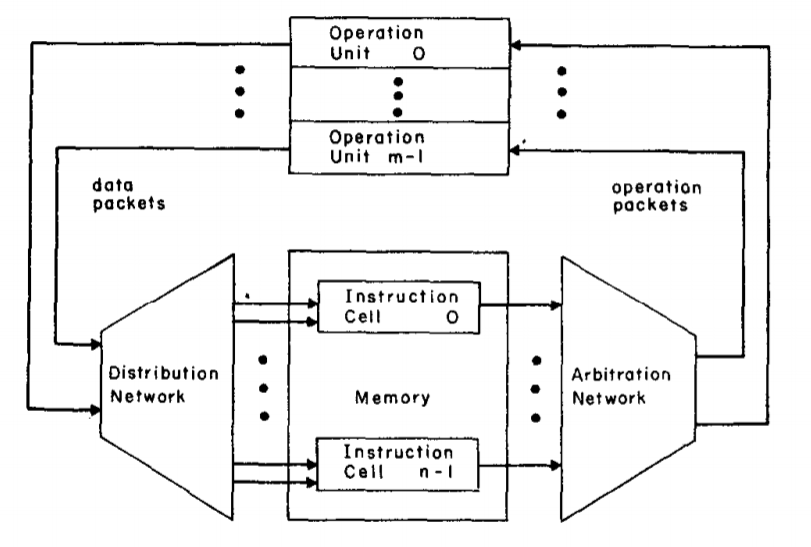
\includegraphics[width=\textwidth,height=8cm]{figures/isca94_elementory_processor.png}
    \end{center}
    \caption{ISCA94 - Elementary Processor.}
    \label{fig:elementory_processor}
  \end{small}
\end{figure}

The Manchester prototype dataflow computer~\cite{DBLP:journals/cacm/GurdKW85} proposed
a powerful dataflow processing engine based on dynamic tagging.
Instructions do not reference memory, since the data-dependence arcs
allow data to be transmitted directly from generating instruction to subsequent instruction.
Consequently, instructions can be viewed as \textbf{pure operations}.
Individual systems differ mainly in the way they handle re-entrant code.
Static systems do not permit concurrent reactivation,
and so they are restricted to implementing loops and cannot accommodate recursion.
Dynamic systems permit recursive reactivation,
either by code-copying or tagging, at every occurrence of re-entry.

The MIT tagged-token dataflow architecture~\cite{DBLP:journals/tc/ArvindN90} proposed
a novel multiprocessor dataflow architecture.
A traditional von Neumann processor has fundamental characteristics
that reduce its effectiveness in a parallel machine:
\begin{compactitem}
  \item its performance suffers in the presence of long memory and communication latencies;
  \item they do not provide good synchronization mechanisms
        for frequent task switching between parallel activities;
  \item it is a significant added complication for the programmer to manage parallelism explicitly.
\end{compactitem}
A token carries the address of an instruction in this fixed code,
and a dynamic context that specifies the frame for a particular invocation of the function.
The format of a token can now be seen: $(c, s, v)_p$.
Here, $c$ is the context, $s$ is the address of the destination instruction, $v$ is the datum,
and $p$ is the port identifying which input of the instruction this token is meant for.
The value $(c, s)$ is called the fag of the token.

\subsection{TRIPS Architecture}

TRIPS architecture~\cite{DBLP:conf/isca/SankaralingamNLKHBKM03} proposed 
a polymorphous dataflow processor using static loop execution model.

Specialized architecture design led to performance fragility,
in which applications incur large swings in performance
based on how well they map to a given design.
One strategy for combating processor fragility is to build a heterogeneous chip multiprocessor (diverse cores).
An alternative approach (easier) is to use multiple heterogeneous processors.
This architectural ``polymorphism'' can defined as the capability to \textbf{configure hardware}
for \textbf{efficient execution} across broad classes of applications.

A key question, is what granularity of processors and memories
on a \textbf{CMP} is best for polymorphous capabilities.
The finer-grained architectures (e.g FPGAs) can offer high performance
on applications with fine-grained (data) parallelism,
but will have difficulty achieving good performance on general-purpose and serial applications.
A synthesis appraoch uses a fine-grained CMP to exploit regular, fine-grained parallelism
and tackles irregular, corse-grained parallelism by
synthesizing multiple processing elements (PEs) into larger ``logical'' processors.

\subsubsection{TRIPS Overview}


\subsection{EDGE Architecture}

EDGE architecture~\cite{DBLP:journals/computer/BurgerKMDJLMBMY04} proposed

\subsection{WaveScalar Architecture}

WaveScalar~\cite{DBLP:conf/micro/SwansonMSO03}\cite{DBLP:journals/tocs/SwansonSMPPMOE07}
makes use of the implementation of loop in dynamic dataflow architecture.

coarse-grained architecture, such as TeraFlux and Runnemede.

\clearpage

\section{Dataflow for AI}

ASIC- or FPGA-based AI-EI chips often use a spatial architecture.
Compared to general-purpose chips, dedicated chips are used
in specific scenarios and their functions are limited.
A simple and regular hardware architecture is the basis for reducing design costs
and is a prerequisite for implementing low-cost dedicated chips.
A low enough chip cost can hedge the limitations of dedicated chip functionality.

The spatial architecture uses Dataflow processing.
In the spatial architecture, the ALU forms a data processing chain
that enables data to be transferred directly between ALUs.
In this spatial architecture, each ALU has its own control logic and local storage (register file).
Among them, the ALU with local storage is defined as PE.

For spatial architectures, hardware design is based on
low-energy memory in hierarchical memory and increases data reuse
(essentially, convolution is spatial reuse, which reuses spatial invariance) to reduce power consumption.
In addition, Dataflow controls data reading, writing, and processing.
In general, the spatial architecture balances I/O and computational problems
based on hierarchical memory and data flow,
thereby reducing power consumption and increasing computational throughput.

In the inference of deep learning, there are a large number of computational requirements.
However, these calculations are performed in a hierarchical order.
Therefore, the control process is relatively simple and clear.
It can be seen that the Dataflow processing method is very consistent
with the computational requirements based on the deep neural network inference part.

The data stream can determine which data is read into which memory and when it is processed.
In addition, there is no randomness in DNN inference.
Therefore, an AI-EI chip based on the fixed architecture of Dataflow
can be designed from the perspective of optimal power consumption.
Currently, most AI-EI chips for deep learning inference use Dataflow.

In hierarchical memory, a large amount of memory read and write operations
consumes much more energy than a small memory.
Thus, once a piece of data has been moved from large memory to small memory,
the data block is reused as much as possible to minimize power consumption.
However, low-power memory has limited storage space.
How to maximize the reuse rate is the most important condition
for designing based on the Dataflow accelerator.
That is, by maximizing the data reuse rate to reduce I/O requirements
and reduce data processing power consumption,
thereby increasing throughput and reducing overall energy consumption.
Common DNN data stream types include: weight fixed data stream, output fixed data stream, No local reuse (NLR), and row fixed data stream.

Weighted fixed data stream: The weight data is read from the DRAM,
placed in the RF of the PE and remains unchanged,
then the input data is broadcasted to each PE,
and finally the part and (partialsum) of the PE array are obtained.
The processing method reduces the number of times the weight data is read from the RF of the PE,
and minimizes the number of times the weight is directly read from the DRAM,
thereby maximizing the multiplexing rate of the convolution
and the weight of the filter to reduce the multiplexing rate and energy consumption.
NeuFlow is an AI-EI chip based on this type of data processing.

Output fixed (OS) data stream: By inputting data in the stream in the PE array
and then broadcasting the weight data to the PE array,
the sum of the parts in the RF is kept constant,
thereby minimizing the energy consumption of the read and write parts.
The Cambrian ShiDianNao is based on an output fixed AI-EI chip.
In addition, depending on the processing target,
the data stream can be divided into OS\_A with the convolution layer as the processing target
and OS\_C with the full connection layer as the processing target.
OS\_B is an OS data stream between OS\_A and OS\_C.

NLR data stream: The RF of the PE array does not store any fixed data.
On the contrary, in this case, all data read and write operations are performed in the global buffer.
The Cambrian DianNao and DaNiaoNao are AI-EI chips based on this data processing method.

Fixed data stream: Maximize all data multiplexing rates and make all data read and write operations in RF as much as possible,
reducing read and write operations on global buffers to reduce power consumption.
Each PE can complete a 1D convolution operation,
and multiple PEs can perform a 2D convolution operation.
In a two-dimensional PE array, the weight data of each row is multiplexed on the PE unit on the horizontal axis,
and the input data of each row is multiplexed on the PE unit on the diagonal line,
and multiple on the vertical axis On the PE unit,
the portion of each row and the data are multiplexed, that is,
the fixed data stream can maximize the multiplexing rate of all data,
thereby optimizing the power consumption globally.
Eyeriss' NPU is based on line-fixed AI-EI chips.

\clearpage

% \begin{table}
%   \begin{small}    
%     \caption{This is for long caption.}
%     \label{tab:table}
%     \begin{center}
%       \begin{tabular}[c]{l|l}
%         \hline
%         \multicolumn{1}{c|}{\textbf{xx}} & 
%         \multicolumn{1}{c}{\textbf{xx}} \\
%         \hline
% 	      a & b \\
% 	      c & d \\
% 	      e & f \\
%         \hline
%       \end{tabular}
%     \end{center}
%   \end{small}
% \end{table}

% \begin{algorithm}
%   \floatname{algorithm}{算法}
% 	\algrenewcommand\algorithmicrequire{\textbf{输入:}}
% 	\algrenewcommand\algorithmicensure{\textbf{输出:}}
% 	\caption{xxxxxxxxxx}
% 	\label{alg:main}
%   \begin{algorithmic}[1]
%     \State \textbf{return} $state$
% 	\end{algorithmic}  
% \end{algorithm}

% \begin{equation}
%   \text{UCT} = \frac{w_i}{s_i} + c\sqrt{\frac{\ln{s_p}}{s_i}}
%   \label{eq:uct}
% \end{equation}

\bibliographystyle{unsrt}
\bibliography{bibs/dataflow}
\addcontentsline{toc}{section}{References}
\newpage

\end{document}
